\documentclass[a4paper,10pt,oneside]{article}
\usepackage[polutonikogreek,italian]{babel}
\usepackage[utf8x]{inputenc}
\usepackage{amsmath}
\usepackage{amsthm}
\usepackage{amssymb}
\usepackage{amscd}
\usepackage{graphicx}
\usepackage{float}
\usepackage{array}
\usepackage{rotating}
\usepackage[small]{caption}
\usepackage{lscape}
\usepackage{fancybox}
\usepackage{booktabs}
\parindent0ex 
\renewcommand{\fboxsep}{0.5cm}
\usepackage{hyperref}
\renewcommand{\textfraction}{0.05}
\renewcommand{\topfraction}{0.95}
\renewcommand{\bottomfraction}{0.95}
\renewcommand{\floatpagefraction}{0.35}
\setcounter{totalnumber}{5}
\restylefloat{figure}
\newlength{\drop}\underline{}
\begin{document}
{\huge Laboratorio cinematica unidimensionale}
\begin{abstract}
 La cinematica, dal greco \textgreek{κινεῖν} (velocità) è quella branca della fisica che si occupa di descrivere il moto degli oggetti a prescindere dalla cause che lo hanno provocato. In questa esperienza andremo  ad osservare il moto unidimensionale di un oggetto e misureremo la sua posizione rispetto ad un sistema di riferimento solidale ai sensori ad ultrasuoni presenti in laboratorio. Utilizzeremo quindi i dati acquisiti per calcolare la velocità e l'accelerazione dell'oggetto.
\end{abstract}


\vspace{2cm}

Il laboratorio di fisica del Liceo Scientifico L.Martin di Latisana dispone di una guidovia a cuscino d'aria che ci permetterà di effettuare misurazioni di moti quasi uniformi e di moti accelerati.

\begin{figure}[H]
 \centering
 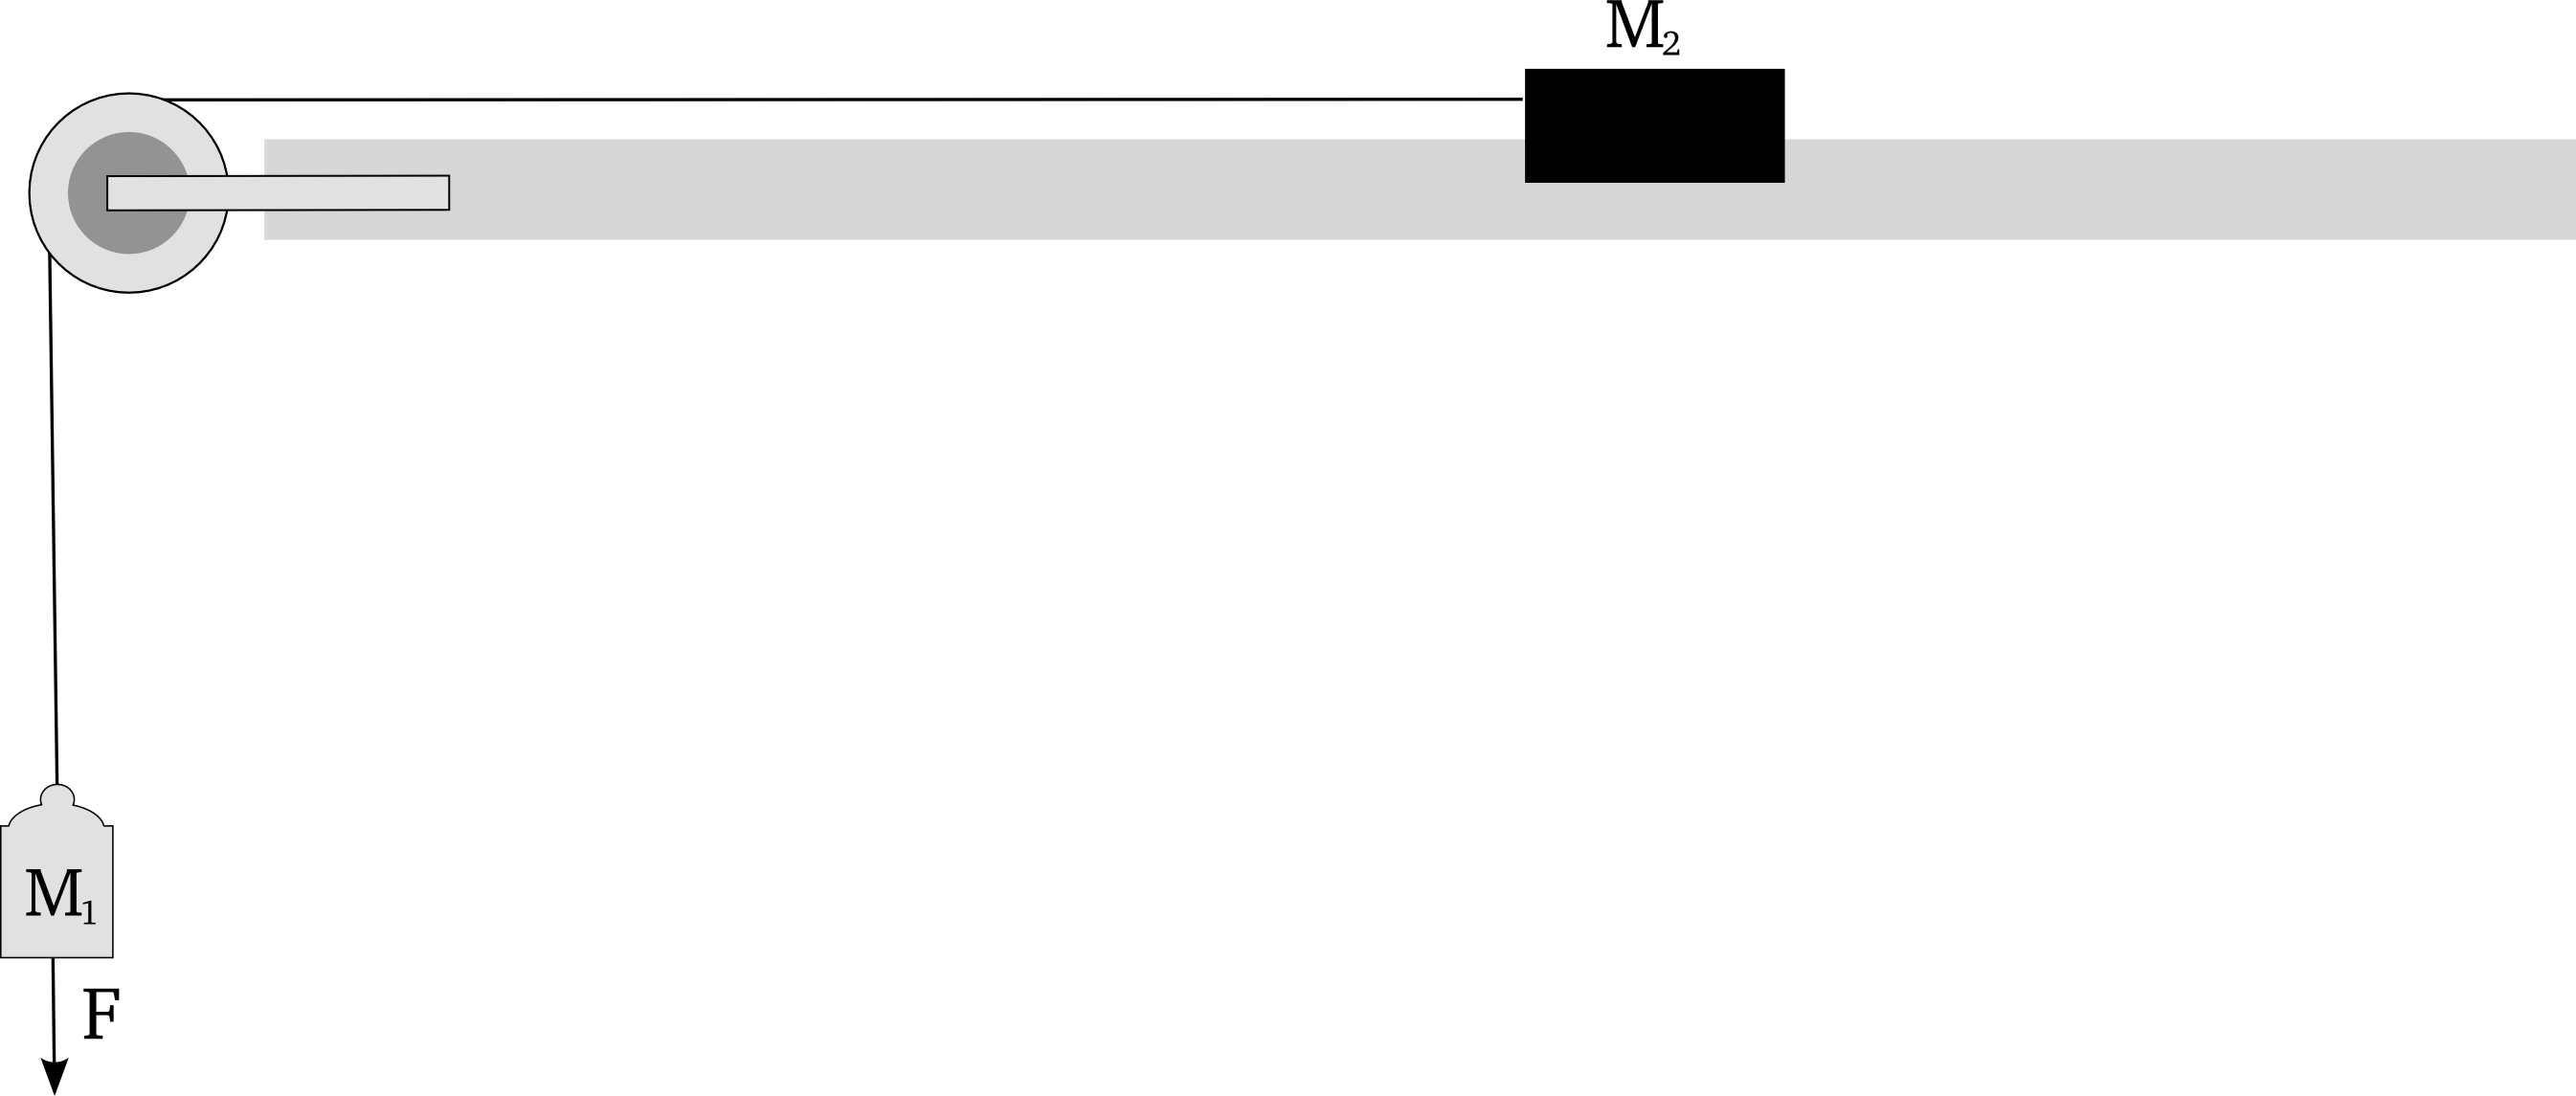
\includegraphics[width=\textwidth]{./guidovia.png}
 % guidovia.png: 3774x1458 pixel, 72dpi, 133.12x51.43 cm, bb=
 \caption{Guidovia a cuscino d'aria con sensori di posizione montati}
 \label{fig:guidovia_cuscino}
\end{figure}

Come sensori di posizione utilizzeremo i \textsl{CI-6742} della Pasco che verranno montati durante l'esperienza di laboratorio lungo la guidovia. In rete è disponibile un \emph{datasheet} completo dei sensori riportante tutte le loro caratteristiche tecniche\footnote{Come esercizio cercate il file pdf con le caratteristiche dei sensori di posizione che potrete poi citare nelle vostre relazioni}.

\begin{figure}[H]
 \centering
 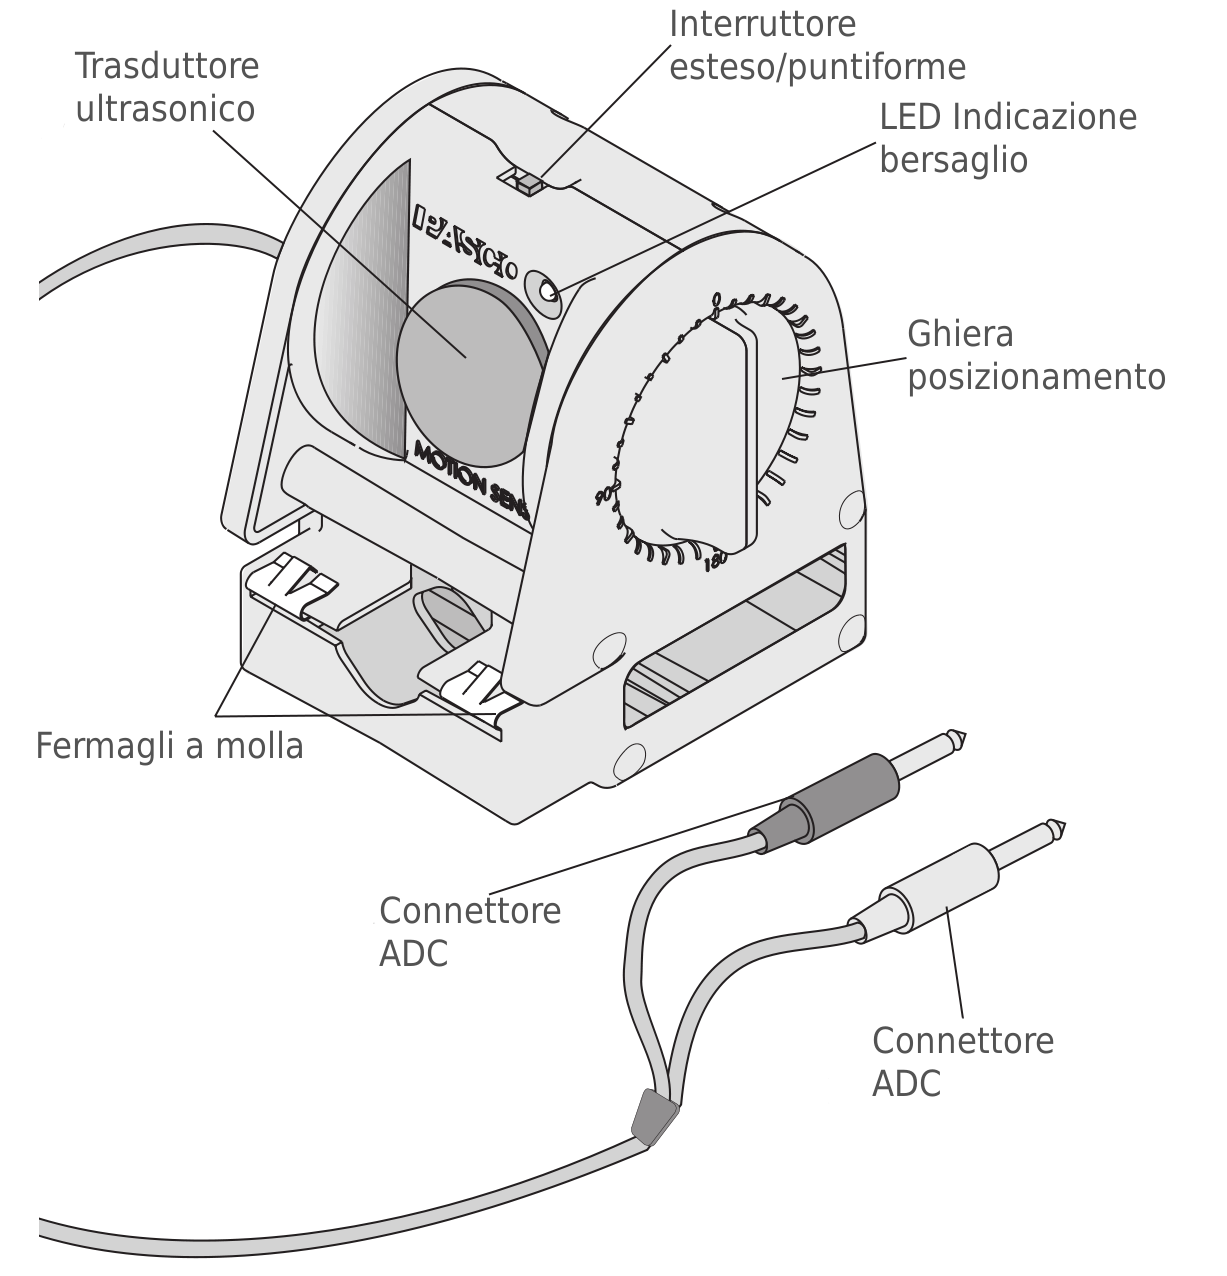
\includegraphics[width=0.8\textwidth]{./sensore_moto_pasco.png}
 % sensore_moto_Pasco.png: 1227x1276 pixel, 300dpi, 10.39x10.80 cm, bb=
 \caption{Sensore di posizione Pasco, disegno tratto dal datasheet della strumentazione}
 \label{fig:Pasco_sensore1}
\end{figure}

Le fasi dell'esperienza saranno indicativamente le seguenti:
\begin{itemize}
 \item Norme per la tabulazione dei dati
 \item Legge oraria e sua rappresentazione grafica
 \item Calcolo numerico di accelerazione e velocità
 \item Utilizzo del software Pasco
 \begin{itemize}
   \item Rappresentazione dei dati
   \item Calcoli sulle traiettorie
   \item Esportazione dei dati
 \end{itemize}
\item Posizionamento dei sensori di posizione
\item Acquisizione dati di moti uniformi e uniformemente accelerati su binario
\item Acquisizione dati su piano inclinato
\end{itemize}

\section{Tabulazione dei dati}

Una corretta tabulazione dei dati è estremamente importante per una chiara presentazione dei valori misurati durante l'esperienza di laboratorio. Le grandezze che andremo a misurare durante questa esperienza sono il tempo ($t$) e la posizione ($x$) rispetto all'origine del nostro sistema di coordinate (il sensore ad ultrasuoni). I dati devono essere riportati con le opportune unità di misura\footnote{Oltre alle unità di misura dovrebbero essere riportate in tabelle le incertezze relative ad ogni valore misurato. I valori riportati non sono di alcuna utilità se non conosciamo l'errore da cui sono afflitti} in una tabella simile alla seguente [\ref{tab:extab1}]:
\begin{table}[H]
\begin{center}
\begin{tabular}{ll}\toprule
$t_i$ & $x_i$\\ \midrule
0.1s & 0.3m\\
0.2s & 0.4m\\
\ldots &\ldots \\ \bottomrule
\end{tabular}\caption{Un esempio di dati misurati durante un esperimento, nota come ad ogni valore riportato sono associate le rispettive unità di misura}\label{tab:extab1}
\end{center}
\end{table}

\section{ Legge oraria e sua rappresentazione grafica}
Dopo aver tabulato i dati andremo a creare un grafico che correla la posizione rispetto all'origine ed il tempo trascorso da quando è partito il cronometro. I dati dovranno essere riportati in un grafico cartesiano ortonormale ed isometrico, con il tempo sull'asse delle ascisse e lo spazio sull'asse delle ordinate. I punti di coordinate $(t_i,x_i)$ ci serviranno per determinare una legge oraria approssimata $x=f(t)$ che meglio si adatta alle nostre misurazioni\footnote{Esistono dei metodi matematici estremamente raffinati per determinare la funzione che meglio si adatta alle nostre misurazioni. Se siete curiosi potete cercare in biblioteca \textsl{Numerical Recipies} di cui potete trovare una versione non molto aggiornata (gratuita) in rete all'indirizzo \url{http://www.nr.com/oldverswitcher.html} }
Per realizzare il grafico potete utilizzare:
\begin{itemize}
 \item Matita e carta millimetrata
 \item OpenOffice.org Calc (foglio elettronico)
 \item Gnuplot \url{www.gnuplot.info}
 \item Scilab \url{www.scilab.org}
 \item Sage \url{www.sagemath.org}
 \item Il software Pasco
\end{itemize}

\begin{figure}[H]
 \centering
 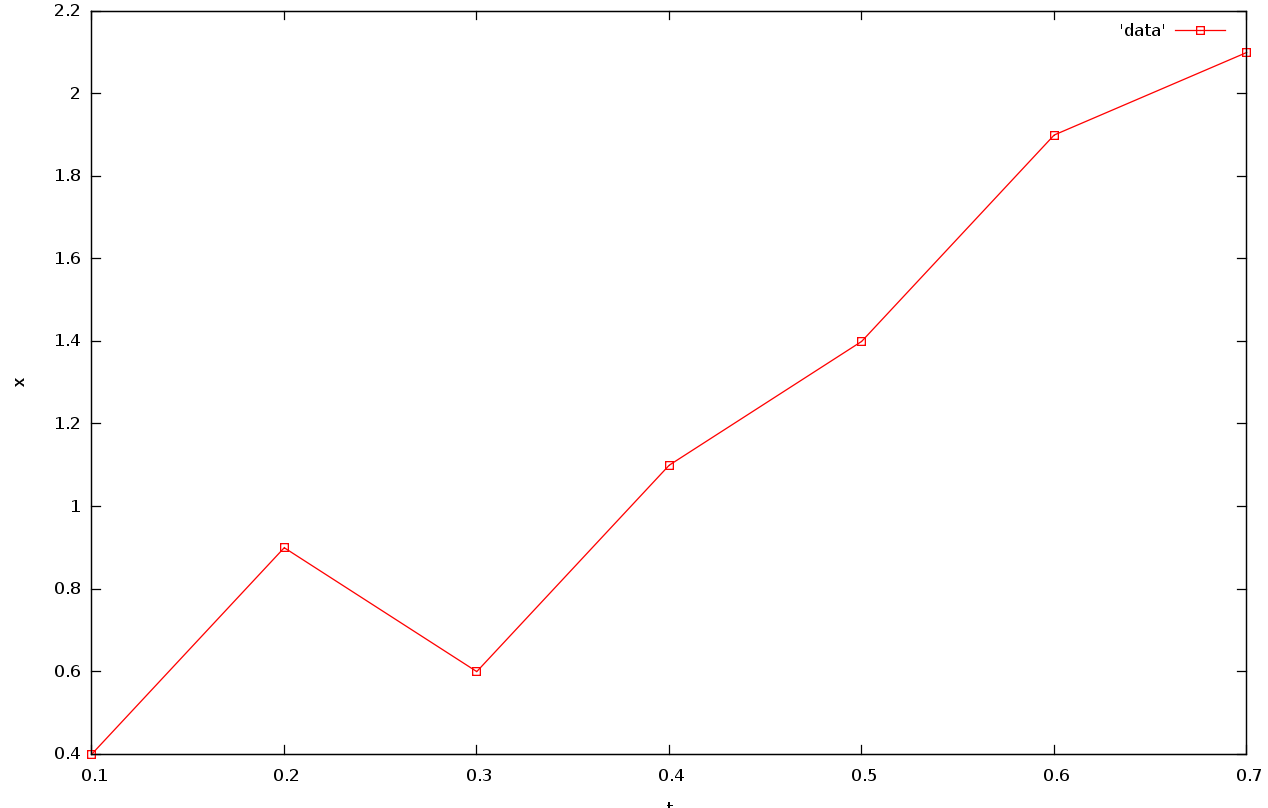
\includegraphics[width=\textwidth]{./gnuplot1.png}
 % gnuplot1.png: 964x572 pixel, 300dpi, 8.16x4.84 cm, bb=
 \caption{Grafico di un insieme fittizio di dati realizzato con Gnuplot}
 \label{fig:gnuplot_1}
\end{figure}


Mentre riportate le misure sul grafico dovrebbe esservi chiaro che la curva che state disegnando (unendo idealmente i punti con una spezzata) \textbf{non} rappresenta la forma della traiettoria ma la dipendenza temporale della posizione dell'oggetto dall'origine del sistema di coordinate. La traiettoria, in questo caso, è unidimensionale dato che la coordinata spaziale che descrive la posizione del corpo è unica.

\section{Calcolo numerico di velocità ed accelerazione}

Il sistema Pasco ci fornisce la posizione del corpo in un dato istante di tempo\footnote{Il software Pasco è anche in grado di calcolare velocità ed accelerazione, non utilizzeremo questa caratteristica del programma in quanto vogliamo imparare ad effettuare il calcolo autonomamente} otteniamo così una lunga lista di coppie $(t_i,x_i)$ siccome il sistema effettua le misurazioni ad intervalli regolari di tempo (da $5\ Hz$ a $120\ Hz$) i nostri dati saranno generalmente esprimibili come $(\Delta t\cdot i,x_i)$ dove l'indice $i$ indica l'i-esima misura.
Dalla teoria studiata in classe sappiamo che:
\begin{equation}
 v_x(t)=\lim _{\Delta t \to 0} \frac {\Delta x}{\Delta t}
\end{equation}
chiaramente questa formula non è applicabile ad un sistema reale dato che non è materialmente possibile effettuare misurazioni della posizione ad intervalli di tempo arbitrariamente piccoli. La velocità che andremo a calcolare sarà quindi rappresentata nel nostro grafico $(t,s)$ dalla pendenza della spezzata che congiunge due punti (misure). Il valore che otterremo dal calcolo sarà quindi una velocità media\footnote{
La formula [\ref{forward_diff}] è detta differenza in avanti utilizzando tre punti (la così detta differenza centrale) è possibile ottenere un risultato più accurato nel calcolo della velocità }:
\begin{equation}\label{forward_diff}
\overline{v}_x(t_i)=\frac{\Delta x}{\Delta t}=\frac{x_{i+1}-x_i}{\Delta t}
\end{equation}
Una volta ottenuta la velocità media possiamo calcolare l'accelerazione media utilizzando una formula analoga alla [\ref{forward_diff}]:
\begin{equation}
 \overline{a}_x(t_i)=\frac{\Delta v}{\Delta t}=\frac{v_{i+1}-v_i}{\Delta t}
\end{equation}
Al termine dei calcoli riporteremo i risultati ottenuti in una tabella e quindi in un grafico che ci aiuterà a visualizzare la dipendenza temporale di accelerazione  e velocità:
\begin{table}[H]
\begin{center}
\begin{tabular}{llll}\toprule
$t_i$ & $x_i$& $\overline{v}_i$& $\overline{a}_i$ \\ \midrule
$0.1s$&$0.3m$&$1ms^{-1}$&$10ms^{-2}$\\
$0.2s$&$0.4m$&$2ms^{-1}$&\ldots\\
$0.3s$&$0.6m$&\dots&\ldots\\
\ldots &\ldots&\dots&\dots \\ \bottomrule
\end{tabular}\caption{Tabella con velocità ed accelerazioni calcolate dalle misurazioni effettuate in laboratorio, notate come con $n$ misure sia possibile calcolare $n-1$ velocità ed $n-2$ accelerazioni}\label{tab:extab1}
\end{center}
\end{table}



\section{Esportazione dei dati da Pasco Data Studio}
Il programma Data Studio, installato nei computer del laboratorio di fisica, ci permette di acquisire le misurarazioni dai sensori di posizione e di effettuare le prime analisi sui dati figura [\ref{fig:pasco_dati1}].
\begin{figure}[H]
 \centering
 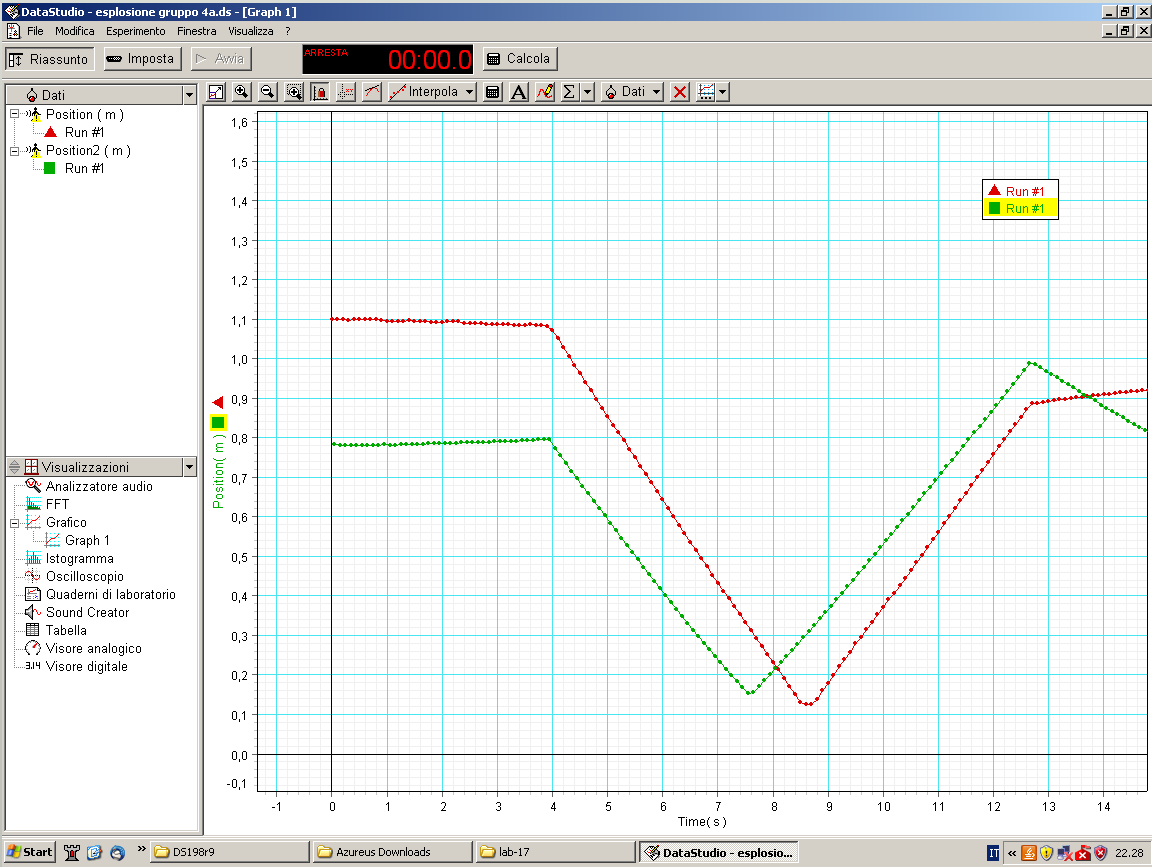
\includegraphics[width=\textwidth]{./pasco2.png}
 % pasco2.png: 1152x867 pixel, 96dpi, 30.48x22.94 cm, bb=
 \caption{Serie dai misure acquisite tramite Pasco Datastudio}
 \label{fig:pasco_dati1}
\end{figure}

Il programma permette l'esportazione dei dati acquisiti  in formato testuale per una successiva analisi manuale o tramite altri software dedicati al calcolo numerico. La procedura di esportazione è molto semplice, dal menu \textsl{File} selezionate \textsl{Esporta dati\ldots} e scegliete quindi l'insieme di misure da esportare figura [\ref{fig:pasco_export}].
\begin{figure}
 \centering
 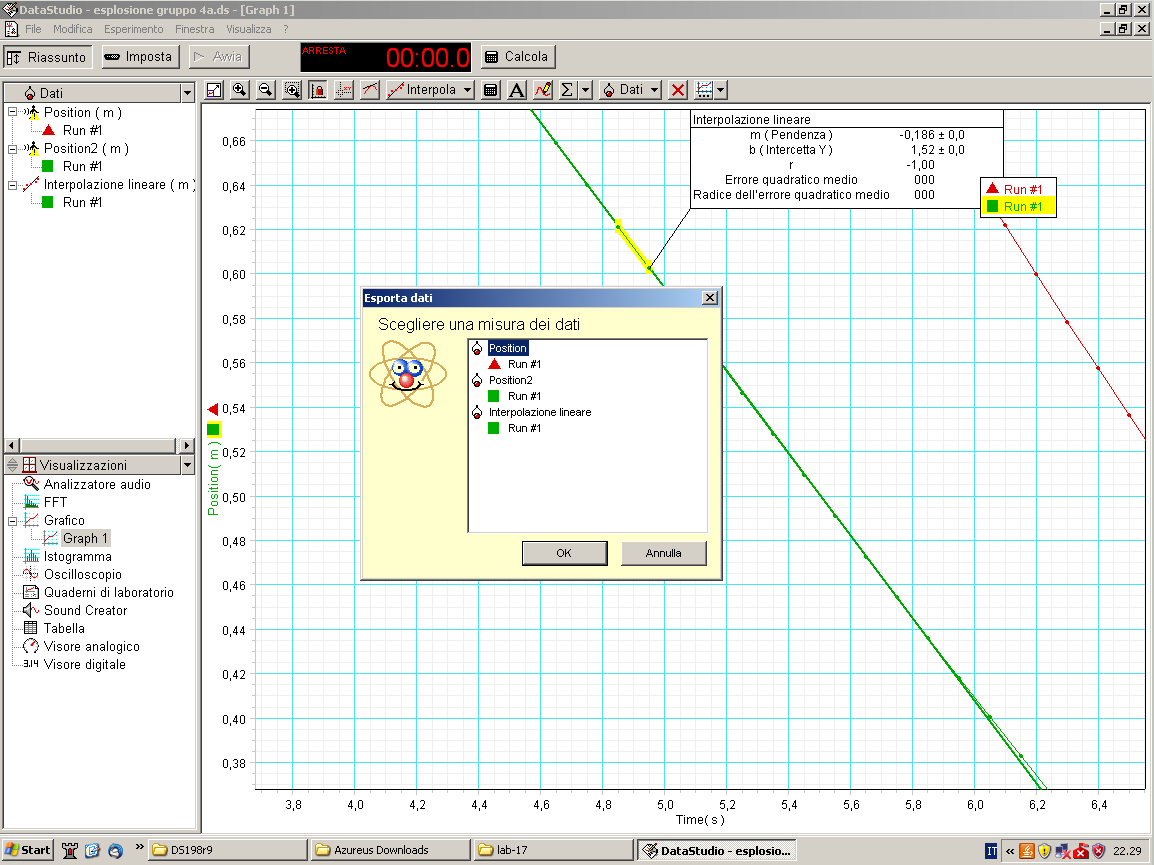
\includegraphics[width=\textwidth]{./pasco3.png}
 \caption{Esportazione dei dati da Pasco Data Studio}
 \label{fig:pasco_export}
\end{figure}

I dati saranno esportati in un file di testo utilizzabile poi da tutti i programmi di analisi numerica:
\begin{verbatim}
Position, Run #1
Time ( s )	Position ( m )
0,0032	1,100
0,1032	1,099
0,2032	1,100
0,3032	1,096
0,4032	1,099
0,5032	1,099
0,6032	1,099
0,7032	1,099
\end{verbatim}



\end{document}
